\chapter{De fora para dentro}

\singlespacing
\begin{flushright}
\textit{"A toda hora,}

\textit{a todo momento}

\textit{De dentro pra fora,}

\textit{De fora pra dentro"}

Walter Franco
\end{flushright}
\doublespacing

Na abordagem ``de fora para dentro'', nossa pesquisa busca entender como novatos são recebidos pela comunidade da Wikipédia. Observamos aqui as estratégias já utilizadas de recepção e replicamos em campo uma delas, as editatonas, para observarmos de perto qual a experiência prática vivida por esses editores.

Nesta frente de pesquisa, foi realizada então uma breve revisão bibliográfica sobre o assunto, uma construção de modelo de atividade para recepção de usuários novatos, a execução deste modelo de atividade no mundo real e inferências quantitativas aos bancos de dados para analisar as atividades realizadas.

\section{Estratégias para recepção de novatos.}

"a ampla aceitação de artefatos e arranjos organizacionais é condição sine qua non para participar de uma comunidade de prática (Lave and Wenger 1991, Star 1996). Estranhos e pessoas de fora de um grupo têm a infraestrutura como um alvo de aprendizado. Novos participantes adquirem familiaridade com estes objetos à medida que se tornam membros do grupo. (STAR; RUHLEDER, 1996, apud BOWKER; STAR, 2007, p.35)" (FEITOSA, 2010. p. 17)

# talvez aproveitar originais da fala acima

# Buscar algo do Primo sobre frustração dos entrevistados dada a dificuldade em colaborar no WP. Citar que essa dificuldade foi observada nas falas de lá, e que iremos atrás de falas da Wikipédia organizando nossas atividades.

\subsection{Coisas dentro da Wikipédia}

Seguindo esta trilha então narramos esforços da comunidade wikipedista de melhorar a recepção de novatos, como o Teahouse (MORGAN e HALFAKER, 2018), espaço na Wikipédia anglófona que funciona como um fórum com tutores e usuários novatos, e o Snuggle (HALFAKER et al., 2014), que segundo a Wikipédia (WiKIPEDIA-PT, “Wikipédia:Snuggle”, 07/07/2014) ”é um sistema web para observação e apoio a novatos [...] desenvolvido para permitir que tutores observem as atividades de usuários recém registrados separando novatos desejáveis (boa fé e produtivo (sic)) de indesejáveis (má fé e vândalos)”, a iniciativa "Wikipedia Adventure" (NARAYAN et al., 2017) e o robô ClueBot NG.


# Dificuldade de usuários novos: vários casos de sucesso da TeaHouse na enwiki, mas na ptwiki o "Café dos novatos", que foi renomeado para https://pt.wikipedia.org/wiki/Wikip%C3%A9dia:Tire_suas_d%C3%BAvidas é muito pouco usado e nada linkado.
# Posso comparar número de uso do café na en e na ptwiki


# Falar sobre Wikipedia Adventure (NARAYAN et al., 2017)
# usar (TARABORELLI e CIAMPAGLIA, 2015) 

\subsection{Outreach}

# “Quando os de dentro saem”. Trazer essa fala do Latour para falar de outreach.
# Falar de forma global do programa de educação, atividades glam e editatonas.

Eu diria ## [[citation needed]] que GLAM e Programa de Educação são as duas grandes linhas de outreach do movimento, e a editatona é uma metodologia que é operada por esses e demais tipos de projetos.
-- Mais que isso, a Editatona junta estruturas internas na Wiki com atividades outreach. Ela une os dois mundos. Isso nos chama atenção para ela

# Falar da existência da wiki de outreach. Da tentativa de compartilhamento de experiências, práticas e resultados em um movimento extensionista global e da ferramenta de compartilhamento de Learning Patterns.
# Quando falar de Learning Patterns lembrar de problematizar o conceito de melhores práticas. “Toda prática é surpreendente”. Cukierman ( PASTEUR ? )

\subsubsection{GLAM}

# Catar alguns autores de outreach para falar sobre glam por alto.

# Trazer números. Falar sobre como muitas vezes as atividades GLAM apoiam outros projetos Wikimedia, como Commons, Wikisource e Wikidata.

# Citar o projeto 1lib1ref.
-- Falar que uma das contribuições da pesquisa foi melhoria do código do citation hunt, e sua disponibilização para pt.
--- Trazer números do citation hunt.

# Citar números dos WL* e mencionar que as ferramentas para monitoramento e avaliação foram criadas pela comunidade brasile

\subsubsection{Programa de Educação}

# sobre pré-programa de educação citar interesse da comunidade de engajar acadêmicos e pesquisa (TARABORELLI 2011)

# Falar sobre a história do programa. Quando foi criado, qual sua capilaridade. Quantos cursos em quantos países, bytes adicionados….
    • Estimula professores a proporem para seus estudantes a edição verbetes da Wikipédia como uma atividade da disciplina.
    • Fundação Wikimedia cria materiais de apoio e estimula voluntários a apoiarem as iniciativas como embaixadores.

# Sobre o programa de educação, usar (MARQUES, 2012), (CARVER et al., 2012), (ARCHUBY, 2018), (SOLER-ADILLON, 2018)

…. Programa de Educação, que aconteceu entre 2011 e 2015, onde podemos observar de forma explícita a dificuldade de professores e estudantes para criar conteúdos na Wikipédia e suas tentativas de negociação com a comunidade para a criação de estratégias que possibilitassem a permanência dos conteúdos criados pelos estudantes no projeto.(MARQUES, 2012).
Sabemos que conteúdos criados em editatonas e em salas de aulas costumam ter dificuldades para permanecer na Wikipédia. São comuns os relatos de professores e alunos desmotivados por verem suas contribuições desaparecerem do ar pouco depois de serem salvas. Os casos mais repetidamente vistos como bem sucedidos adotam estratégias para tentar mitigar essa situação, como por exemplo estimular os alunos a editar primeiro em uma página de testes, onde o conteúdo será revisado pelo professor e por outros voluntários, para só então ser adicionado à página do verbete desejado. 

Assim por exemplo foi feito por Juliana Bastos Marques, professora da UNIRIO, responsável pelo primeiro caso de instanciamento do Programa de Educação da Wikimedia Foundation no Brasil. Como relatado por ela na Revista História Hoje (2012, p. 339), "uma maneira bastante segura de evitar conflitos com wikipedistas durante a realização da disciplina é fazer que os alunos escrevam seus artigos apenas em suas páginas de teste, e que após a avaliação eles sejam corrigidos pelo/a professor e embaixadores, para que então possam ser ‘colocados no ar’. Este modelo não é consenso entre os professores que adotaram o projeto até agora, mas se provou fácil e seguro". Corroborando com nossa experiência, a autora afirma no mesmo texto que “observou-se que outros cursos já ministrados no Brasil dentro do mesmo projeto não conseguiram alcançar resultados satisfatórios no mesmo grau" (MARQUES, 2012. p. 338).

# Discussão é rica para quando for falar do programa de educação é sua extensão pro MediaWiki, da necessidade de medir, e da criação de ferramentas para gestão / monitoramento dos cursos.
- Se for falar disso, trazer fala de Zé Marcos. O SI parece feito pensando na demanda de quem está no centro de poder por dados, e não no uso cotidiano dele. Os usuários parecem "perder tempo" preenchendo campos que gerarão relatórios que não são de seu interesse. Pq afinal preencher corretamente então?
# Citar Latour sobre a discussão anterior:
"[...] construir centros implica trazer para eles elementos distantes – permitir que os centros dominem à distância –, mas sem trazê-los "de verdade" [...] Esse paradoxo é resolvido criando-se inscrições que conservarão, simultaneamente, o mínimo e o máximo possível, através do aumento da mobilidade, da estabilidade ou da permutabilidade desses elementos. Esse meio termo entre presença e ausência muitas vezes é chamado de informação. Quando se tem uma informação em mãos, tem-se a forma de alguma coisa sem ter a coisa em si. Como sabemos, essas informações (ou formas, ou formulários, ou inscrições – todas essas expressões designam o mesmo movimento e resolvem o mesmo paradoxo) podem ser acumuladas e combinadas nos centros"(LATOUR, 2000, p. 396)" p. 17

\subsection{As Editatonas}

# Falar aqui que é uma forma de atividade que perpassa atividades de educação, de glam, wiki projetos e outras iniciativas avulsas, inclusive tendo Learning Patterns "próprios", compartilhados por extensionistas de diversas frentes do movimento.

Uma das principais formas que o Movimento Wikimedia tem para engajar e trazer novos/as usuários/as à comunidade são as editatonas. Realizadas por todo o mundo, são eventos onde pessoas se reúnem para editar sobre um mesmo tema de interesse. Como definida pela própria enciclopédia, no verbete ``Maratona de edição'' na Wikipédia em português, uma editatona é um evento ``\textit{durante o qual editores se reúnem para editar e melhorar um tema ou tipo específico de conteúdo, geralmente incluindo um treinamento em edição básica para novos editores. A palavra é uma combinação das palavras ``editar'' (\textit{edit}) e ``maratona'' (\textit{marathon})}'' \citewiki{ptwiki_maratona}.
# Editatonas: falar da ambiguidade do termo em inglês e da perda na tradução.

# trazer foto de uma editatona

Existem variações em seu formato, mas normalmente a atividade começa com um (ou mais) editor/a(es/as) experiente(s) apresentando o funcionamento da enciclopédia e introduzindo suas políticas editoriais. Em sequência, os/as demais participantes criam uma conta de usuário/a e começam a escrever, individualmente ou em grupo, verbetes de seu interesse. Nesta fase, o/a(s) usuário/a(s) experiente(s) atua(m) como tutor/a(es/as), tirando dúvidas dos/as novatos/as que apareçam durante o processo de edição.

Existem também algumas editatonas que funcionam como ``forças-tarefas'' de usuários experientes melhorando verbetes sobre um determinado assunto focal, como por exemplo ``patrimônio natural brasileiro''\footnote{https://pt.wikipedia.org/wiki/Wikipédia:Edit-a-thon/Atividades\_em\_português/Wiki\_Loves\_Earth\_Brasil\_2015 , acessada em 19 de março de 2020.} ou ``eleições no Brasil''\footnote{https://meta.wikimedia.org/wiki/Programa\_Catalisador\_do\_Brasil/2013-2014/Micro-subsídios/Solicitação/Wikitona\_Eleições\_2014 , acessada em 19 de março de 2020.}. Estas atividades dispensam a explanação inicial, e, os/as presentes, editores/as já experientes, partem rapidamente para a divisão de tarefas e escrita de conteúdos. Habitualmente, essas forças tarefas são realizadas online, e a maioria das editatonas presenciais é direcionada em apresentar o mundo wiki a novos/as editores/as a partir de assuntos que sejam de seu interesse.

No início de 2020, a página para divulgação de editatonas da Wikipédia em português já contava com 120 eventos cadastrados desde 2013, sendo 115 deles (98,5\%) realizados no Brasil (\citewiki{ptwiki_edit_a_thon_atividades_portugues}). Já na página para editatonas da Wikipédia em inglês, estavam mapeados 121 eventos, com o primeiro datando de janeiro de 2011 e o último de maio de 2018 (\citewiki{enwiki_how_run_edit_a_thon}), indicando que provavelmente essa comunidade passou a registrar seus eventos realizados no último ano e meio em outro lugar. Já a Wikipédia em espanhol apresentava 92 eventos (\citewiki{eswiki_editaton}), mas aparentemente México, Argentina e Espanha, pólos movimentados de atividade wiki, estão com seus números desatualizados. Terminando nosso passeio pelas páginas sobre editatonas das maiores Wikipédias do mundo, encontramos 60 atividades mapeadas na versão francófona (com destaque para um evento realizado recentemente em Guiné, o primeiro fora do eixo França-Canadá) (\citewiki{frwiki_journées_contributives}) e 83 na enciclopédia em alemão (\citewiki{dewiki_edit_a_thon}).

Se por um lado nossa breve busca não conseguiu números precisos sobre a quantidade de editatonas realizadas pelo mundo, entendemos que os valores encontrados já são suficientes para indicar a relevância deste tipo de evento para o Movimento Wikimedia. Eles também indicam que, além da organização destes eventos ser uma estratégia muito utilizada por todo o mundo, ela é especialmente popular no Brasil.

# Para falar de editatonas citar (CAMPANY e KAHILI-HEEDE, 2018), (FARZAN et al. , 2016), (LITTLEJOHN, Allison et al., 2019), (MARQUES e LOUVEM, 2013)



\section{Organizando nossas editathonas}

A fim de estudar a dificuldade de entrada de novos/as usuários/as \textit{in loco}, em nossa abordagem de pesquisa ``de fora para dentro'', resolvemos organizar nossas próprias editatonas como atividades de campo. Podendo assim observar problemas encontrados pelos/as participantes, e mapear com eles/as os mecanismos de governança da Wikipédia que se apresentam como barreiras, muitas vezes intransponíveis, deixando novatos/as bem intencionados/as sem saber como prosseguir.

Com isto, partindo das observações feitas \textit{in loco} nas editatonas, regressamos a bancada de ciência de dados de nosso laboratório. Nela andamos colados ao banco de dados, realizando inferências nos dados abertos da Wikipédia. Investigamos padrões, elementos e comportamentos da governança da comunidade que interagiram com nossos participantes durante e após as editatonas.

\subsection{Por que resolvemos fazer editatonas?}

*** talvez falar também sobre a escrita dos 3 verbetes sobre autores CTS. ## Pegar notas e citações no card do Trello sobre trabalho do Esocite. ver https://trello.com/c/y6cDtTZi/290-adicionar-sobre-trabalho-do-esocite-no-cap%C3%ADtulo-4

A metodologia adotada de realizar editatonas foi validada como pertinente logo no início da pesquisa em 2017, com a realização de uma atividade em sala de aula com a turma de pós-graduação da disciplina ``\textit{Estudos CTS (Ciências-Tecnologias-Sociedades): aproximações brasileiras e latino-americanas}'', ministrada no Programa de Engenharia de Sistemas e Computação da COPPE/UFRJ, no 2º período de 2017. Atividade esta que teve seus resultados retratados no trabalho ``\textit{Práticas de escrita biográfica na Wikipédia em português em turmas de pós-graduação}'', apresentado no VII Simpósio Nacional de Ciência, Tecnologia e Sociedade (Esocite.BR), também em 2017 (\cite{andrade_historias_2017}).

A editatona foi realizada durante uma aula em que o professor não poderia estar presente, e os/as estudantes deveriam se auto organizar e autogerir para realizar alguma atividade. Inicialmente o grupo imaginava que iria trabalhar no CTS Brasil Blog, site idealizado para escoar produções feitas ao longo do curso. Mas, no momento do encontro, percebeu-se que a produção deste já tinha seu fluxo de trabalho remoto bem definido, e que as horas que teríamos juntos presencialmente poderiam ser melhor aproveitadas de outra forma.

Assim, com a decisão de realizarmos uma editatona, fiz uma apresentação sobre o funcionamento da Wikipédia e suas políticas editoriais. Propus então para o grupo que o escopo da atividade fosse o desenvolvimento de verbetes biográficos sobre os autores CTS que estávamos estudando\footnote{No capítulo 4 detalhamos as práticas de escrita biográfica que já estavam ocorrendo durante a disciplina.}. O grupo então debateu sobre quais verbetes editar, e entendendo que existia um artigo que precedia os biográficos em importância para divulgação do tema CTS, definiu que seria feita uma força tarefa para melhorar apenas um verbete: ``\textit{Estudos de ciência, tecnologia e sociedade}''. Os 13 presentes então se dividiram em grupos, responsáveis por criar/melhorar diferentes seções do verbete em paralelo, que somadas comporiam a nova versão do verbete ao final da aula.

Antes da atividade, o verbete contava com 3.989 bytes\footnote{Unidade de medida utilizada pela comunidade para medir o tamanho de revisões e verbetes.}, com uma breve introdução e uma seção textual intitulada ``Ensino'', seguida por seções de ``Bibliografia'' e ``Ligações externas''. Três horas depois, o texto já apresentava 23.570 bytes, sendo 20.281 bytes adicionados pela turma e 18 bytes adicionados pelo usuário FSogumo, que não era aluno do curso e adicionou, durante a atividade, o \textit{template} de geração automática de referências ao verbete, que agora contava com dez seções textuais diferentes.

Sabendo da dificuldade tão relatada de conteúdos criados em salas de aula persistirem por um longo período de tempo na Wikipédia (\cite{marques_trabalhando_2012}), (\cite{carver_assigning_2012}), (\cite{archuby_experiencias_2018}), (\cite{soler-adillon_wikipedia_2018}), voltamos então ao verbete ``\textit{Estudos de ciência, tecnologia e sociedade}'' um mês depois da realização da atividade, para pesquisar o que teria acontecido com as edições de nossos/as editores/as.

Encontramos mais três edições feitas por alunos da turma no verbete após a atividade, adicionando mais 10.551 bytes, e percebemos uma situação que contradiz toda a literatura sobre editatonas: nenhuma edição de nossa turma havia sido revertida, e todo o conteúdo criado por nossos/as novos/as editores/as continuava no ar. Este fato é ainda mais surpreende pois em nossa atividade os/as estudantes foram estimulados/as a editar diretamente a Wikipédia, sem realizar uso prévio das páginas de testes, o que diminuiria ainda mais as chances de sobrevivência de seus conteúdos (\cite{marques_trabalhando_2012}).

Perante tão distinta situação, resolvemos então investigar o que havia acontecido de especial em nossa editatona, e enredamos a ferramenta \textit{Objective Revision Evaluation Service} (ORES)\footnote{Em português Sistema Objetivo de Avaliação de Revisões.}, para analisar todas as edições feitas durante a atividade.

O ORES é uma ferramenta de inteligência artificial que avalia edições (também chamadas pelos/as usuários/as de revisões) feitas nas Wikipédias. Solicitamos aqui de nossos/as leitores/as a gentileza de aceitar o ORES como uma caixa-preta (assim como ela é aceita pelos/as editores/as e reversores/as das Wikipédias)\footnote{Na verdade no uso cotidiano da enciclopédia o ORES faz parte das redes que sustentam outras caixas pretas, enquanto ele fica invisível fazendo suas avaliações no backend e seu nome permanece desconhecido para a maior parte da comunidade.}, e tomemos suas saídas como avaliações confiáveis sobre as edições apreciadas. Para cada edição, o ORES nos indica probabilidades de ser danosa, feita em boa fé e de ser revertida (``apagada'').

\begin{center}
\begin{table}
\begin{tabular}{ |c|c|c|c| } 
 \hline
\textbf{Id da Edição} & \textbf{Não danosa} & \textbf{Feita em boa fé} & \textbf{Deve ser revertida} \\
\hline
49529742 & 76\% & 87\% & 65\% \\
\hline
49529756 & 76\% & 90\% & 33\% \\
\hline
49529775 & 52\% & 59\% & 71\% \\
\hline
49529792 & 36\% & 35\% & 76\% \\
\hline
49529803 & 80\% & 84\% & 58\% \\
\hline
49529830 & 58\% & 61\% & 73\% \\
\hline
49529836 & 24\% & 34\% & 76\% \\
\hline
49529856 & 42\% & 56\% & 69\% \\
\hline
49531419 & 54\% & 63\% & 72\% \\
\hline
\textbf{49531652} & \textbf{98\%} & \textbf{99\%} & \textbf{04\%} \\
\hline
49781518 & 91\% & 96\% & 12\% \\
\hline
49785059 & 86\% & 88\% & 41\% \\
\hline
49802969 & 67\% & 88\% & 32\% \\
\hline
Média & 64\% & 72\% & 52\% \\
 \hline
\end{tabular}
\caption{Avaliação feita pelo ORES de todas as edições feitas na atividade, com a edição do coordenador destacada em negrito.}
\label{table:avaliacao-ores}
\end{table}
\end{center}

A tabela \ref{table:avaliacao-ores} exibe a avaliação do ORES para todas as edições feitas no contexto de nossa editatona, começando da mais recente e descendo cronologicamente. Observando a tabela podemos notar que a maioria de nossas edições foram vistas pelo sistema tanto feitas em boa fé como não danosas, mas apresentavam percentual alto de chances de serem revertidas.

Não por acaso, esse é exatamente o perfil de edição que organizadores de editatonas relatam vivenciar. Seus/suas colegas estão editando em boa fé e realizando alterações que não são danosas para a enciclopédia, mas a falta de um determinado padrão de escrita, esperado pela comunidade, faz com que as edições sejam revertidas.

Ao observarmos atentamente a tabela criada pelo ORES uma edição nos salta aos olhos. A edição com id \textbf{49531652} apresenta 98\% de chances de não ser danosa, 99\% de ser feita em boa fé e apenas 4\% de chances de ser revertida. Ao clicar no detalhamento desta edição, podemos ver que ela havia sido feita pelo usuário experiente que coordenava a atividade (eu), e, nesta edição de 839 \textit{bytes}, todos os conteúdos criados nas edições anteriores eram revisados, sendo colocados no formato wikipédico, com ligações internas e referências no padrão wiki.

Esta edição específica, além de auxiliar a manter na enciclopédia os conteúdos que, segundo o ORES, tinham grandes chances de serem revertidos, estrutura o verbete e ajuda os próximos editores a criarem conteúdos mais ``aceitáveis'' para enciclopédia. As três edições seguintes a essa, feitas por alunos da turma, observam suas chances de serem revertidas caírem drasticamente. Antes da edição do coordenador da atividade, as edições dos novatos apresentavam em média 65,88\% de chances de serem revertidas. Já as realizadas por esse mesmo recorte de usuários/as posteriormente apresentam uma enorme queda nesse valor, para apenas 28,33\%.

Percebemos, então, a importância do coordenador da atividade não ser um mero tutor que orienta os participantes e apresenta dicas de edição. Sua participação ativa na escrita coletiva dos mesmos verbetes que os/as editores/as novatos/as estiverem trabalhando pode auxiliar a manter as edições destes/as no ar, aumentando o sucesso da atividade tanto na satisfação dos participantes, como na disponibilização de mais conteúdos livres a longo prazo.

Após a alta frequência de edições feitas pela turma em agosto e setembro de 2017, a página ``\textit{Estudos de ciência, tecnologia e sociedade}'' voltou a ser pouco editada. Nos dois anos seguintes, até o final de 2019, foram feitas apenas duas contribuições com adição substancial de conteúdo, que não dialogaram com o conteúdo criado pela turma, mas criaram uma seção sobre o ``movimento CTSA (Ciência, Tecnologia, Sociedade e Ambiente)''. Essas edições adicionaram 1415 bytes ao verbete, que permaneceram no ar não revisados nem contestados até o início de 2020.

Esse baixo volume de revisões no verbete mostra a importância das editatonas para não apenas apresentar o funcionamento da Wikipédia buscando engajar novos/as editores/as, como também para produzir conteúdos em assuntos que não sejam muito populares entre os/as editores/as habituais. Apesar de suas mais de 200 mil edições por mês, a Wikipédia tende a concentrar seu maior volume de edições em tópicos como política, esportes ou televisão.

\begin{center}
\begin{table}
\begin{tabular}{ |c|c| } 
 \hline
\textbf{Verbete} & \textbf{Edições em 2019} \\ 
\hline
Big Brother Brasil 19 & 581 \\ 
\hline
Governo Jair Bolsonaro & 357 \\ 
\hline
Copa São Paulo de Futebol Júnior de 2019 & 265 \\ 
\hline
Rompimento de barragem em Brumadinho & 247 \\ 
\hline
Primeira Liga de 2018–19 & 217 \\ 
\hline
Copa da Ásia de 2019 & 197 \\ 
\hline
Campeonato Mundial de Handebol Masculino de 2019 & 182 \\ 
\hline
Lista de participantes do Big Brother Brasil & 173 \\ 
\hline
Verão 90 & 168 \\ 
\hline
Temporada do Sport Club Corinthians Paulista de 2019 & 163 \\ 
 \hline
\end{tabular}
\caption{Lista de verbetes mais editados em 2019 na Wikipédia em português.}
\label{table:verbetes-mais-editados-2019}
\end{table}
\end{center}

Assim, conteúdos criados em editatonas que tenham como temática assuntos não midiáticos tendem a não receber muitas colaborações posteriores, e a produção gerada na atividade tenderá a se estabilizar como o conteúdo que futuros leitores terão acesso em suas pesquisas. Cabe dar bastante ênfase aqui ao fato de que, ao contrários de trabalhos científicos, que ``\textit{a maioria nunca é lida por ninguém}'' (\cite[p.59]{latour_ciencia_1987}), os artigos criados na Wikipédia tem uma grande audiência. E, quanto mais conteúdos tenha um verbete, mais facilmente ele será encontrado por robôs e indexado por mecanismos de busca, fazendo com que ainda mais leitores encontrem o texto.

Com isso, quando uma editatona expande um verbete, além de estar melhorando a qualidade daquele conteúdo para a audiência esperada, ela está também aumentando o público que terá acesso àquele verbete.

\begin{figure}[H]
    \centering
    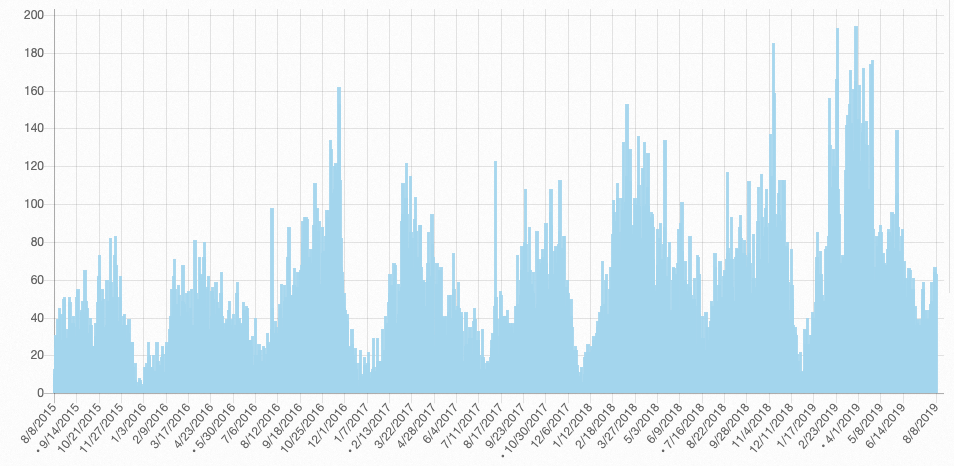
\includegraphics[width=1\textwidth]{Images/acessos-estudos-cts.png}
    \caption{Acessos ao verbete trabalhado dois anos antes e dois anos depois da atividade.}
    \label{fig:acessos-estudos-cts}
\end{figure}

Na figura \ref{fig:acessos-estudos-cts} observamos os acessos ao verbete ``\textit{Estudos de ciência, tecnologia e sociedade}'' entre 8 de agosto de 2015 e 8 de agosto de 2019, exatamente dois anos antes e dois anos depois da editatona. Diferente do trabalho apresentado em 2017 (\cite{andrade_historias_2017}), que observara dois meses antes e dois meses depois da atividade, optamos por esse recorte maior de tempo para dar conta da sazonalidade observada nos acessos ao verbete ao longo do ano, que parece ser bastante influenciada pelo calendário escolar anual.

Compreendido então o recorde, observamos que, nos dois anos anteriores à editatona, o verbete apresentava uma audiência média de 38 acessos por dia. Nos dois anos seguintes, esse número cresce 55,26\%, para 59 acessos diários.

Em valores absolutos, e considerando que o verbete manteria um volume estável de visitas com seu conteúdo anterior\footnote{Consideração benevolente, pois entre 2016 e 2019 os acessos à Wikipédia em português como um todo caíram 1,5\%, como pode ser visto em https://stats.wikimedia.org/\#/pt.wikipedia.org/reading/total-page-views/normal|bar|2016-01-01~2020-01-01|~total|monthly , acessada em 19 de março de 2020.}, isso significa que a editatona de 3 horas, com 13 participantes, proporcionou em dois anos 15.330 leituras a mais sobre ``Estudos de ciência, tecnologia e sociedade'' em português.

Perante o volume de acessos da Wikipédia, aproximadamente 13 milhões por dia somente em português, essas 15 mil leituras em dois anos podem parecer poucos relevantes. Mas, dentro de seu nicho específico de um assunto não muito midiático como ``Estudos de ciência, tecnologia e sociedade'', esse número significa que, no mundo real, 15 mil pessoas que antes não teriam encontrado esse conteúdo em português sobre o tema agora o terão, e com encontrando um texto enciclopédico com maior abrangência e mais referências do que eram apresentadas antes da editatona.

A título de comparação, podemos olhar para os números de outra atividade desenvolvida pela mesma turma: o ``CTS Brasil Blog''\footnote{Disponível em https://ctsbrasilblog.wordpress.com/ .}. Ao longo de todo o curso, os/as estudantes criaram conteúdos e os publicaram nesta página, dedicada especialmente a ``\textit{circular vídeos, resenhas, entrevistas, manifestos e o que mais sair das digestões feitas durante a disciplina}'' (\cite{cts_brasil_blog}). Ao final do curso, o site contava com 17 publicações, feitas por 10 autores/as diferentes.

No ano de sua criação o blog teve seu pico de acessos, muito provavelmente ocasionado pelas visitas dos/as próprios/as estudantes-autores, com 526 visitas. No ano seguinte, este número cai para 215 e, em 2019, o blog encerra o ano com 149 visualizações. Enquanto o volume de acessos inicial pode ser explicado pelos autores acessando o site durante a disciplina, pois só nos dois primeiros meses de vida o \textit{site} recebeu 482 visualizações, os meses seguintes de novembro e dezembro somados totalizam 44 visitas. Podemos então considerar que em outubro de 2017 o blog é estabilizado por seus/suas autores/as, que param de publicar após o término da disciplina, e que os acessos que acontecem a partir daí seriam feitos por leitores/as alheios ao curso. Assim, considerando todos os acessos dos dois últimos meses de 2017, e os anos inteiros de 2018 e 2019, no que podemos considerar leituras orgânicas\footnote{Em mídias sociais, esse é o termo utilizado para acessos feitos sem pagamento de divulgação, por usuários que encontram o site através de links externos ou buscadores.} do conteúdo, temos um volume de 408 visualizações, em uma média de 0.51 visitas por dia.

\begin{figure}[H]
    \centering
    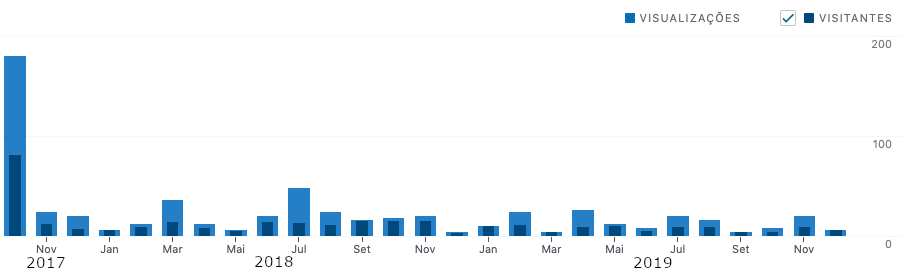
\includegraphics[width=1\textwidth]{Images/acessos-cts-brasil.png}
    \caption{Acessos ao CTS Brasil Blog por mês.}
    \label{fig:acessos-cts-brasil}
\end{figure}

Essa iniciativa do CTS Brasil Blog é claramente um caso de sucesso de divulgação científica, que continua no ar até hoje apresentando para leitores lusófonos, e em grande maioria (89,3\%, como pode ser visto na figura \ref{fig:acessos-geo-cts-brasil}) do Brasil, conteúdos sobre os Estudos de Ciências-Tecnologias-Sociedades, que outrora ficariam restritos às salas de aula de pós-graduação. Mas, seu relevante volume de acessos parece pequeno se comparado às mais de 15 mil visitas que receberam os conteúdos criados na editatona realizada pela mesma turma.\footnote{É importante destacar que o blog aceitava diferentes tipos de conteúdos, e não apenas textos enciclopédicos. Aqui comparamos seus acessos não para medir qual atividade teve maior sucesso, mas apenas para colocar o alcance da atividade realizada na Wikipédia em perspectiva.}

\begin{figure}[H]
    \centering
    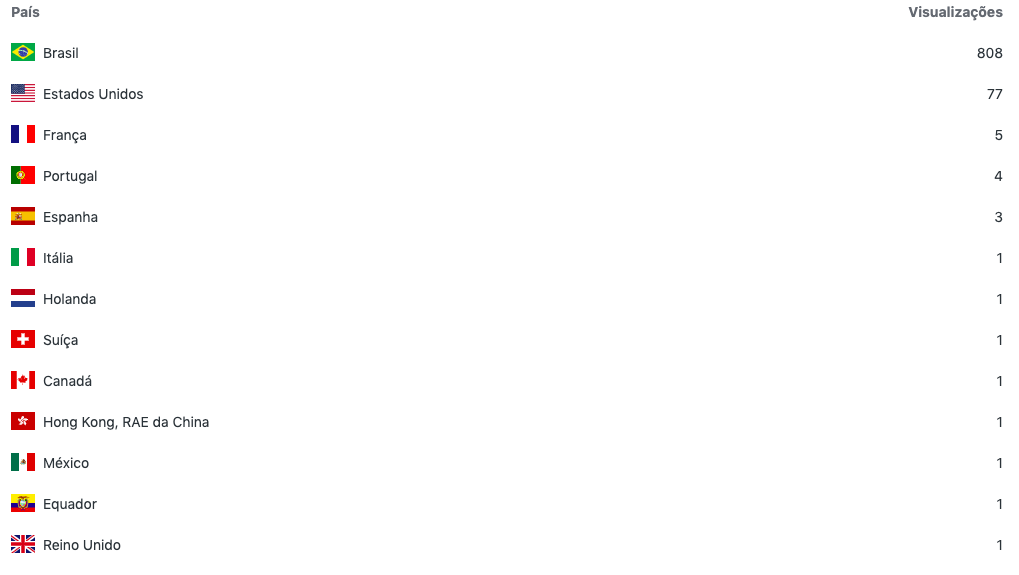
\includegraphics[width=1\textwidth]{Images/acessos-geo-cts-brasil.png}
    \caption{Acessos Geolocalizados ao CTS Brasil Blog.}
    \label{fig:acessos-geo-cts-brasil}
\end{figure}

Tendo em mente estes casos de sucessos na criação de conteúdos, que são de fato lidos pela sociedade além dos muros da universidade, decidimos que convidaríamos para participar das editatonas de nossa pesquisa as redes que orbitam o Laboratório de Informática e Sociedade (LabIS) da COPPE/UFRJ, fazendo com que nosso trabalho de campo tenha um efeito colateral um tanto quanto interessante: enquanto estudamos os mecanismo de governança da Wikipédia, criamos conteúdos livres em português sobre assuntos relacionados a Ciências-Tecnologias-Sociedades locais, tais como moedas sociais, softwares para acessibilidade, educação popular, informática e educação, mobilização política em redes sociais e demais assuntos que interessarem aos participantes das atividades. Promovemos assim maior acesso de leitores/as do idioma português, por todo o mundo, a esses conteúdos muitas vezes ignorados nos meios de divulgação científica e marginalizados por grande veículos de comunicação.

\subsection{Preparando nossas editatonas}

Nossa pesquisa tinha como objetivo organizar editatonas presenciais para tanto acompanhar in loco, com o olhar míope da formiga, como as interações entre novatos e enciclopédia acontecem, como para disponibilizar livremente em páginas bastante visitadas conteúdos sobre assuntos relacionados a pesquisas do campo CTS e correlatos.

A ideia de organizar editatonas fora validada de forma ad hoc em uma atividade realizada no início da jornada do autor neste curso de mestrado, dentro de uma disciplina oferecida em 2017, antes mesmo do projeto desta tese ter tomado seu recorte atual.

\subsubsection{utilizando Learning Patterns}

Nos preparativos para a realização desta editatona estudamos diversas outras já realizadas, conforme explicitado na seção anterior, e performamos uma extensa revisão bibliográfica dos chamados Learning Patterns da comunidade Wikimedia.

\begin{figure}[H]
    \centering
    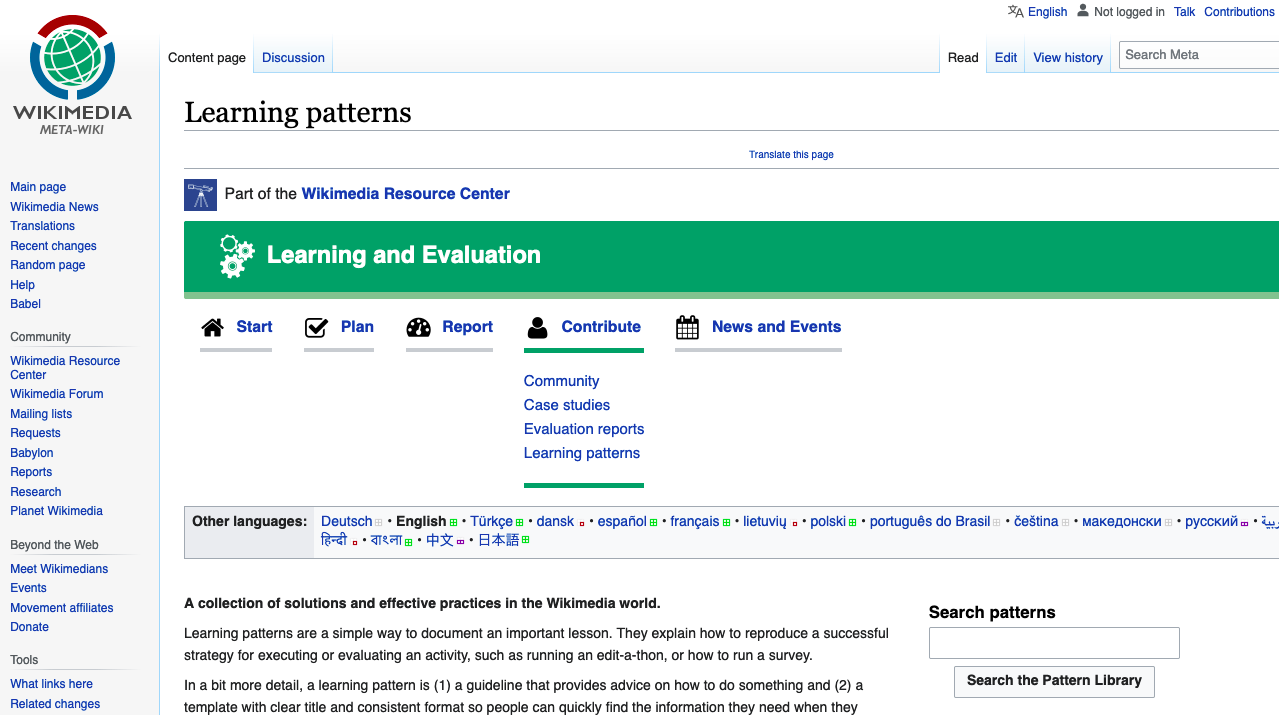
\includegraphics[width=1\textwidth]{Images/learning_patterns.png}
    \caption{Portal de Learning Patterns do movimento Wikimedia.}
    \label{fig:learning_patterns}
\end{figure}

*** Falar da existência da wiki de outreach. Da tentativa de compartilhamento de experiências, práticas e resultados em um movimento extensionista global e da ferramenta de compartilhamento de Learning Patterns.
*** Quando falar de Learning Patterns lembrar de problematizar o conceito de melhores práticas. “Toda prática é surpreendente”. Cukierman ( PASTEUR ? )

*** versar sobre learning patterns criados pela comunidade que foram lidos para a confecção do roteiro. Ver https://trello.com/c/t9SxjmTz/253-encontrar-dados-sobre-learning-patterns-utilizados

*** catar referência sobre o projeto de learning patterns

*** Quando falar de Learning Patterns lembrar de problematizar o conceito de melhores práticas. “Toda prática é surpreendente”. Cukierman

*** Dar números de quantos learning patterns foram lidos neste levantamento.

*** Citar explicitamente os learning patterns utilizados para criar nosso roteiro. Tenho isso mapeado em algum lugar, não sei se no drive ou no trello.

\subsubsection{Criando nosso Learning Patterns}

*** Falar do roteiro criado...ver https://trello.com/c/dH13LfQh/466-detalhar-a-cria%C3%A7%C3%A3o-do-meu-roteiro-da-organiza%C3%A7%C3%A3o-de-uma-editatona
*** ver cards no trello da coluna "o que fazer a cada editatona". Falar de dados, prazos, emails convite...

Seguindo a trilha dos learning patterns estudados, criamos predefinições\footnote{Predefinições são página do MediaWiki que funcionando como templates, podendo ser importadas para outras páginas trazendo automaticamente uma estrutura previamente determinada.} para facilitar a utilização das páginas de testes pelos participantes das editatonas. Estas predefinições permitiram com facilidade a criação e listagens de novas subpáginas de testes, tarefa nada trivial para um usuário não habituado ao funcionamento do MediaWiki.

\begin{figure}[H]
    \centering
    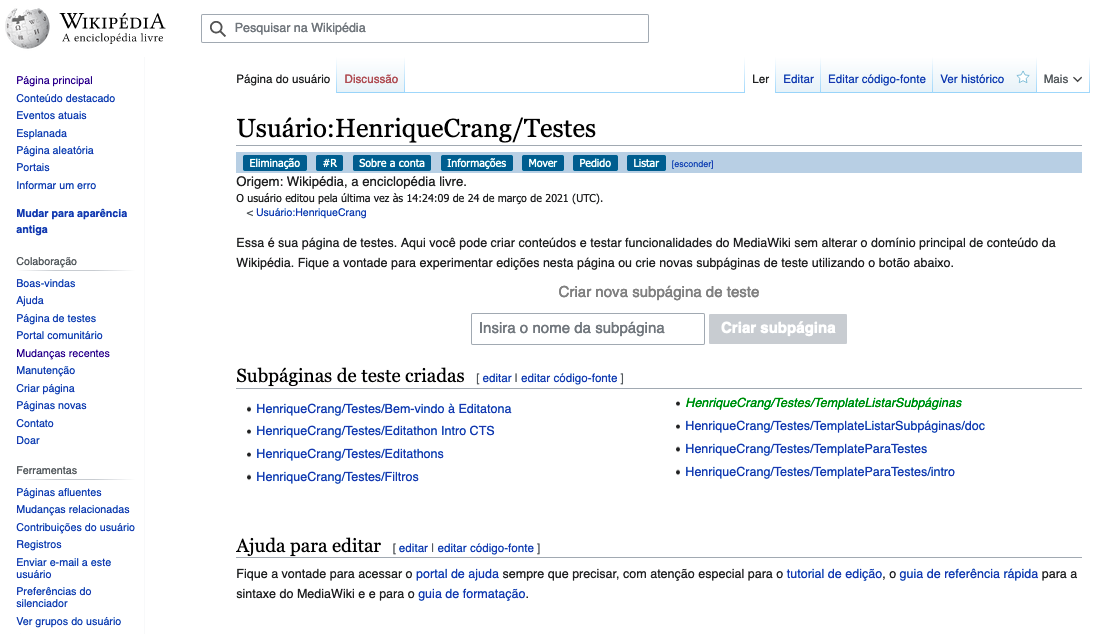
\includegraphics[width=1\textwidth]{Images/pagina_de_Testes.png}
    \caption{Página de testes criada utilizando a predefinição desenvolvida pela pesquisa.}
    \label{fig:pagina_de_testes_editatona}
\end{figure}


*** Sobre Criação de pré-definições... ver https://trello.com/c/Mp3HXAPg/187-documentar-trabalho-feito-criando-pr%C3%A9-defini%C3%A7%C3%B5es

*** Usar mais prints para mostrar as pre-definições


A predefinição se chama "Predefinição:Página de testes do usuário", e atualmente é utilizada por XX usuários da Wikipédia em português. \footnote{Como pode ser visto em https://pt.wikipedia.org/wiki/Especial:Páginas_afluentes/Predefinição:Página_de_testes_do_usuário, acessada em }

\subsection{Colocando o plano em prática}

***  Falar aqui da primeira editatona, feita presencialmente em 21 de novembro de 2019.

\begin{figure}[H]
    \centering
    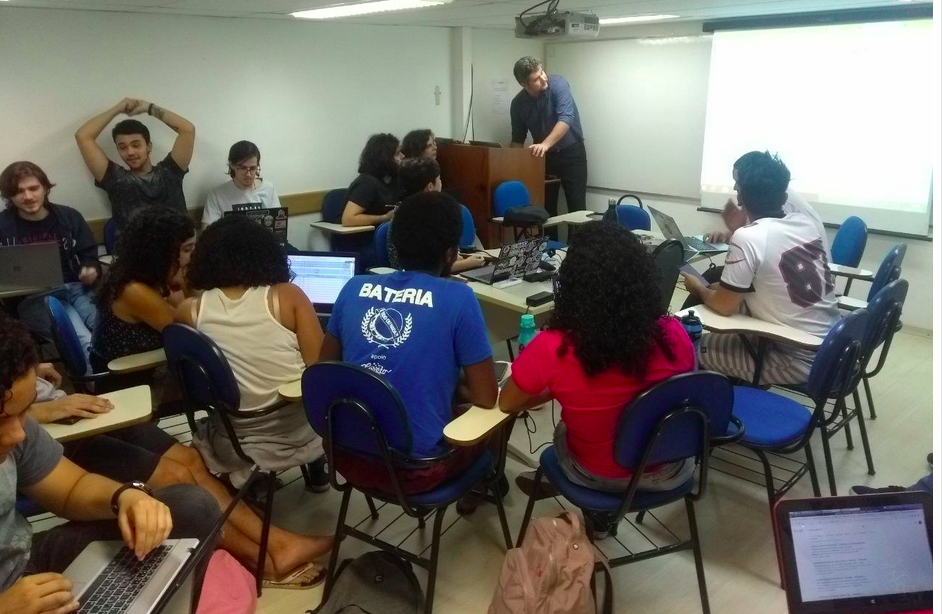
\includegraphics[width=1\textwidth]{Images/editatona_presencial.png}
    \caption{Editatona presencial com turma de graduação no dia 21 de novembro de 2019.}
    \label{fig:editatona_presencial}
\end{figure}

***  Trazer alguns poucos números dela, e concluir dizendo que essa foi a única realizada seguindo o mapa original, pois a realidade se mostrou mais realista que o plano, e desvios e adaptações foram necessários para que a pesquisa continuasse em um mundo que mudou da noite para o dia


\subsubsection{No meio do caminho tinha uma pandemia}

Após a validação de nosso roteiro com a editatona realizada ao final de 2019, nos planejamento para realizar diversas atividades no início do primeiro semestre letivo de 2020. Porém, o mundo foi surpreendido pela pandemia de COVID-19, que se apresentou acompanhada de medidas de isolamento social que inviabilizaram a realização de mais atividades presenciais conforme planejado.

"em qualquer caso de trabalho acadêmico, os planos de pesquisa sonhados pelo pesquisador têm poucas chances de serem realizados em sua totalidade." (GONÇALVES, 2016. p. 18)

*** atividades foram adiadas duas três vezes... passado um tempo, percebemos que não era uma mera questão de adiar o plano, mas de o alterar para dialogar com essa nova realidade que se impôs.

Assim, nossa pesquisa encontrou um bloqueio, e se viu obrigada a buscar desvios negociando com o vírus SARS-CoV-19, com as políticas públicas de isolamento social, com softwares de videoconferência e com redes de engajamento popular à distância para construir novas composições e seguir, se não para o rumo previsto originalmente, mas para um novo que apontasse para um norte (ou seria sul?) próximo à discussão proposta no trabalho.

Partimos então para a criação de uma nova metodologia de realização de editatonas com novatos, que pudesse ser realizada à distância. Conforme já mencionado, tradicionalmente as editatonas focadas em novatos são realizadas presencialmente e os eventos à distância reúnem editores experientes. Desta forma, toda a literatura existente sobre editatonas à distância não nos foi de muita valia, por suas metodologias sempre partirem do princípio de que os participantes já dominam o funcionamento do MediaWiki e as políticas editoriais da Wikipédia.

Subitamente percebemos que nossa pesquisa ganhara uma nova dimensão e responsabilidade: caberia a nós propormos e testarmos uma metodologia nova para a realização de editatonas para editores novatos à distância. Debruçamo-nos então sobre este desafio e passamos a testar diversas ferramentas de realização de encontros virtuais e a frequentar eventos online organizados por diversas instituições para encontrarmos exemplos e inspirações.

*** necessidade de tradução, translação..sabemos que traições acontecerão no processo, mas buscamos o máximo de fidelidade ao propósito e à propiciar dinâmicas entendidas como interessantes.

Uma das características marcantes das editatonas presenciais com novatos é a escrita em conjunto, no mesmo teclado, de textos. Pequenos grupos de 2 a 4 pessoas se formam em torno de um computador e, juntos, os participantes enfrentam os desafios de escrever verbetes enciclopédicos pela primeira vez. Como seria possível mimetizar esta experiência virtualmente? Como no mundo online, mesmo estando todos na mesma sala virtual, é possível a formação de pequenos que dialogam entre si, sem que a conversa de cada grupo atrapalhe os demais?

Em salas convencionais de videoconferência esta prática seria inviável. Diferente de uma sala do mundo físico, onde diferentes pessoas podem falar ao mesmo tempo para grupos diferentes e todos serem compreendidos, em uma sala virtual é imprescindível que apenas um participante fale por vez, sob pena do encontro se tornar uma cacofonia incompreensível.
Cogitamos então criar várias salas virtuais, dividir os participantes em grupos e pedir para que cada um se dirigisse a um link diferente após uma abertura realizada em uma única sala. Porém, não estávamos confortáveis com esta solução. A necessidade de abrir uma nova conexão durante a atividade parecia algo um tanto quanto desmobilizante, e que criaria uma segregação entre os grupos impedindo uma série de dinâmicas interessantes de colaboração e circulação observadas em editatonas presenciais.

Umas das dinâmicas que se perderiam seria a troca de grupo. É normal um novato querer circular pela sala em uma editatona. A pessoa pode começar em um grupo, mas durante a editatona se engajar em outra atividade. Algumas vezes este movimento acontece pois a pessoa escuta, de rabo de ouvido, algum comentário vindo de outro grupo que a faz querer contribuir com outra tarefa.

Outra dinâmica muito dificultada pela segregação das salas seria o apoio do wikipedista experiente. Em editatonas presenciais, ele roda entre os grupos, apoiando e tirando dúvidas, e pode a qualquer momento ser chamado por um grupo que necessite ajuda. Mesmo que o usuário experiente tivesse acesso aos links de todas as diferentes videoconferências e ficasse pulando de sala em sala, como um grupo que precise de ajuda em um determinado instante poderia chamá-lo? Seria necessário utilizar outra ferramenta, como o telefone por exemplo, ou o grupo precisaria aguardar mais alguns minutos para a aparição surpresa do tutor em sua sala virtual, tal qual um enfermo acamado agoniadamente aguarda pela rara ronda médica.

Ademais, em editatonas presenciais não são incomuns momentos em que o wikipedista experiente, a partir da dúvida de um grupo específico, compartilha com todos os presentes alguma situação que o grupo tenha vivido, explicando a questão para todos e dando dicas sobre como prosseguir quando a mesma barreira porventura for encontrada por qualquer dos participantes.

A possibilidade de inviabilizar todas as dinâmicas narradas acima nos causou grande inquietação, pois sentíamos que a editatona virtual que estávamos criando não seria capaz de oferecer uma boa experiência aos participantes.

\subsubsection{Encontrando uma tradução viável}

Em nosso esforço para traduzir a metodologia de editatonas presenciais para novatos ao mundo virtual, sem que as traições que inevitavelmente aconteceriam no processo inviabilizassem a atividade, enxergamos uma luz ao fim do túnel quando testamos a ferramenta Discord.

O Discord é um serviço de comunicação online que oferece ferramentas de interação em texto, áudio e vídeo, assim como compartilhamento de tela, e pode ser acessado tanto através de seu aplicativo próprio como através de um webapp em seu site. Criado em 2015 pela produtora de jogos virtuais Hammer \& Chisel, se tornou rapidamente muito popular entre gamers e, com sua popularidade, passou a ser utilizado por outras comunidades e grupos de interesse, ultrapassando em meados de 2019 a marca de 250 milhões de usuários. (SHERR, 2019)

Ao testarmos o Discord uma diferença marcante para outras ferramentas de reuniões virtuais saltou aos olhos: seus espaços de encontro não são orientados a salas, mas a “servidores". No contexto do uso da ferramenta, o termo “servidor” significa um ambiente virtual ao qual os usuários se conectam, e dentro dele podem existir várias salas, tanto de texto como de áudio/vídeo. Estando em um servidor, qualquer usuário consegue navegar por todas as salas de texto sem precisar abandonar a sala áudio/vídeo em que estiver no momento, podendo também, se desejar, trocar de sala multimídia automática e imediatamente com apenas um clique.

\begin{figure}[H]
    \centering
    
\includegraphics[width=0.5\textwidth]{Images/discord_channels.png}
    \caption{Estrutura das salas criadas no servidor “Editatona na Wikipédia” no Discord.}
    \label{fig:estrutura_discord}
\end{figure}

 O dinamismo possibilitado pelo Discord nos deixou esperançosos, e partimos para a criação e personalização de um servidor lá para nossas atividades. Criamos inicialmente cinco salas multimídias, que na interface do sistema rebatizamos de “Salas de encontro”. A primeira chamada “Palestra de abertura”, onde todos os participantes deveriam se encontrar no início da atividade, e as salas seguintes com nomes como “Grupo 1”, com o numeral sendo incrementado a cada sala nova.
 
 Para as salas de texto, chamadas na interface de “Chats em texto” criamos inicialmente seis. Uma com o mesmo nome de cada grupo, uma intitulada “chat-geral” e por fim uma chamada “links-permanentes”, onde somente o organizador poderia enviar mensagens.
 
 Em torno desta estrutura foi criada a seguinte metodologia para desenvolvimento da atividade: todos os usuários, nos convites enviados para a atividade, foram orientados a entrar na sala “Palestra de abertura” assim que acessassem o servidor. Lá, o wikipedista experiente faria uma apresentação de no máximo meia hora sobre a Wikipédia, introduzindo suas políticas editoriais e a interface do sistema MediaWiki. Após a apresentação, os usuários seriam convidados a acessar o chat “links-permanentes”, clicarem em “Criar uma conta”, e depois informarem no “ chat-geral” seu nome de usuário.
 
 Vencido o primeiro contato com a Wikipédia, os participantes então eram convidados a acessar a página criada para organizar os esforços daquela editatona, com link disponível no chat “links-permanentes”. Nessa página, os participantes encontrariam uma lista com sugestões de verbetes a serem trabalhados, lista esta preparada previamente pelo wikipedista experiente e por um representante do grupo que participa da editatona.
 
 Todos são então convidados a debater, em voz ainda na sala “Palestra de abertura” ou em texto no “chat-geral” para os que não puderem/quiserem utilizar microfone, sobre a lista proposta de verbetes a serem trabalhados, que se apresenta apenas como uma sugestão inicial e pode ser totalmente alterada pelos participantes.

\begin{figure}[H]
    \centering
    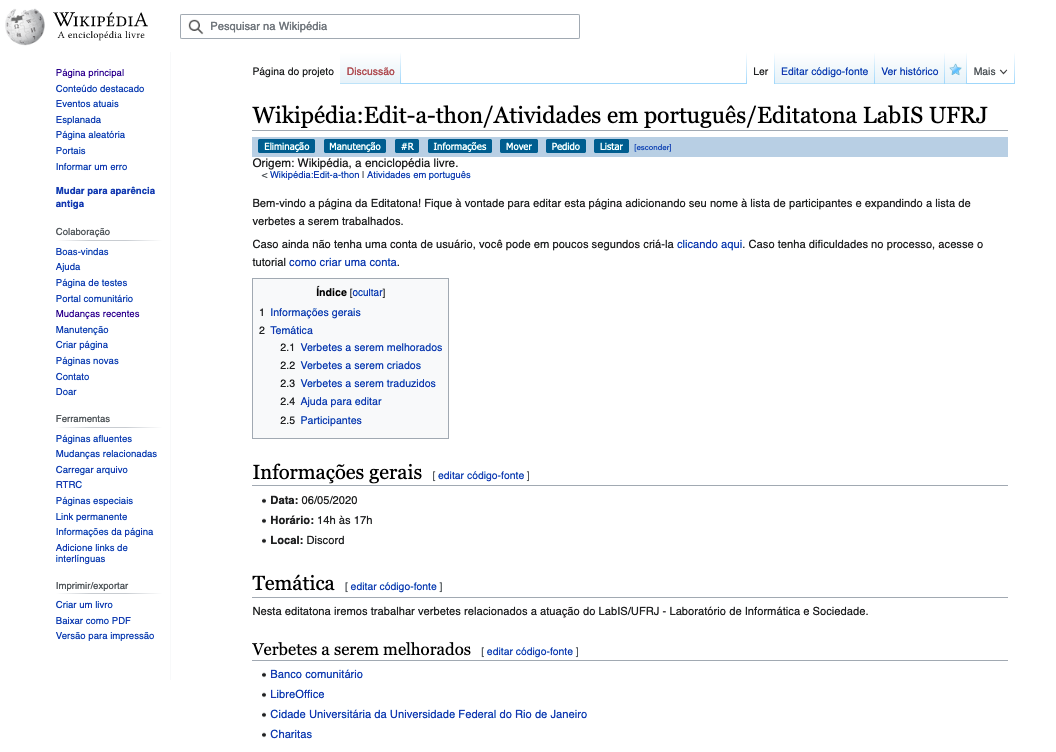
\includegraphics[width=1\textwidth]{Images/pagina_editatona.png}
    \caption{Página de organização de uma das editatonas realizadas durante a pesquisa com lista prévia de sugestões de verbetes a serem melhorados.}
    \label{fig:pagina_editatona}
\end{figure}

 Feita a discussão de quais temas serão trabalhados, o wikipedista experiente então edita o nome das salas que seguiam o padrão ``Grupo X'', adicionando em seus títulos quais temas serão trabalhados em cada sala. Os participantes são então convidados a clicarem no grupo que desejarem, e a sala ``Palestra de abertura'' é esvaziada.
 
 Neste momento começa de fato a escrita enciclopédica, e o wikipedista experiente passa a rodar entre os grupos para auxiliá-los. Para dar conta da escrita coletiva em computadores distintos, os grupos recebem a sugestão de utilizar a ferramenta Etherpad para escrita de seus rascunhos, antes das páginas de Testes da Wikipédia. O MediaWiki, software que gerencia a Wikipédia, não possui funcionalidades que apoiem a escrita ao vivo de textos por duas pessoas que estejam em máquinas diferentes. Isto não é um problema para editatonas presenciais, onde os novatos compartilham o mesmo teclado, mas para a atividade virtual seria muito desmobilizante pedir para um usuário esperar outro editar e salvar uma página de testes para somente então poder editar também.
 
O Etherpad é um software livre que oferece a possibilidade de usuários criarem simultaneamente textos online. Seu funcionamento guarda muitas similaridades com a ferramenta Google Docs, já amplamente conhecida por usuários da Internet. (ARRINGTON, 2008) Optamos por sugerir aos participantes das editatonas a utilização do Etherpad, e não da ferramenta da Google, por ele ser mais leve e não requerer autenticação dos usuários para editar.

Assim, o usuário experiente cria um pad (nome de uma página dentro do Etherpad) para cada grupo, e compartilha o link de cada um no chat de texto dentro do servidor do Discord de cada respectivo grupo.

\begin{figure}[H]
    \centering
    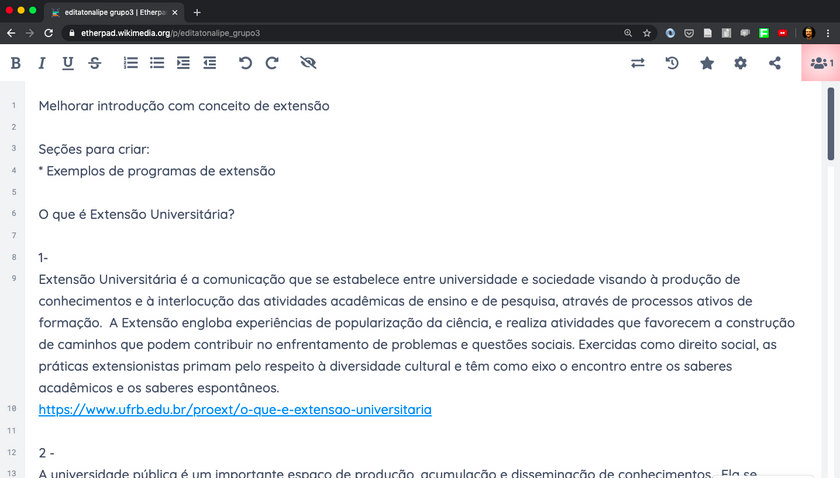
\includegraphics[width=1\textwidth]{Images/etherpad.png}
    \caption{Exemplo de um pad utilizando por um grupo durante uma editatona virtual.}
    \label{fig:etherpad}
\end{figure}

Os membros de cada grupo então são convidados a seguir o seguinte método: escrever no pad o rascunho do texto que irá para a Wikipédia e compartilhar no chat de texto do grupo no Discord links que possam ser utilizados como referências e demais conteúdos relacionados ao processo de escrita do grupo. Desta forma, além do trabalho do grupo ficar estruturado, participantes de demais grupos poderão acompanhar com facilidade o que estiver acontecendo no grupo, colaborando e até mudando de grupo com facilidade se desejarem.

\begin{figure}[H]
    \centering
    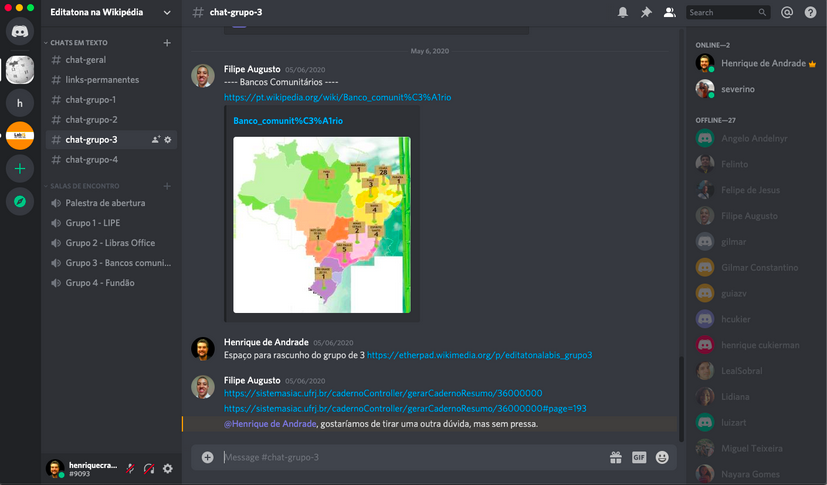
\includegraphics[width=1\textwidth]{Images/discord_full.png}
    \caption{Chat em texto de um grupo das editatonas virtuais, onde podem ser vistos o link para o pad sendo compartilhado e posteriormente um participante pedindo a presença do wikipedista experiente.}
    \label{fig:discord_chat}
\end{figure}

Após duas horas de produção de conteúdo, o wikipedista experiente roda todos os grupos uma última vez, os auxiliando a salvar seus conteúdos e convidando todos os participantes a retornarem para a sala "Palestra de abertura", onde é realizado um bate-papo final com todos, com cada grupo contando para os demais o que foi produzido, como foi a experiência e quais dificuldades encontraram no processo.

\subsection{Acompanhando as editatonas virtuais}

*** Ver https://trello.com/c/AzsF0ayG/450-reaproveitar-texto-sobre-contropedia-quando-come%C3%A7ar-a-apresentar-dados-das-minhas-editatonas

\subsubsection{Escolha dos grupos}

Para a realização, das editatonas foram convidados grupos próximos à linha de pesquisa de Informática e Sociedade da COPPE/UFRJ, que estivessem mobilizados virtualmente durante a pandemia, para editarem verbetes sobre seu assunto de interesse.

Esta escolha de convidados pode ser considerada um movimento de interessamento mútuo da pesquisa. Ao mesmo tempo que essas são redes já mobilizadas e com proximidade facilitante ao pesquisador que conduziu as atividades, os assuntos de interesse desses grupos seriam expandidos na enciclopédia são caros à linha de pesquisa onde este trabalho é realizado, tornando assim a escolha destes grupos para a realização das atividades um tanto quanto óbvia e oportuna.
 Foram então realizadas três editatonas virtuais com os seguintes coletivos da UFRJ: Laboratório de Informática e Sociedade (LabIS), Laboratório de Informática para Educação (LIpE) e Núcleo de Solidariedade Técnica (SOLTEC).
 
\subsubsection{Seguindo as Editatonas}

A primeira editatona com a metodologia virtual foi realizada com a equipe do Laboratório de Informática para Educação (LIpE), contando com a presença de 10 pessoas. Nesta atividade foram criados três grupos, focados em melhorar e escrever verbetes sobre as seguintes temáticas: "linguagem de programação Logo", "extensão universitária" e "história do LIpE".

Já a editatona realizada com o Laboratório de Informática e Sociedade (LabIS) teve a participação de 09 pessoas novas, além de dois membros do LIpE que haviam participado da primeira atividade e retornaram para seguir editando sobre a "história do LIpE". Assim, além do grupo que perdurou da atividade anterior, foram criados novos grupos para tratar dos temas "Libras Office", "bancos comunitários" e "Ilha do Fundão". Nesta atividade contamos com a participação de dois editores que haviam participado também de nossa atividade presencial com a turma de ECI em 2019.2, e puderam compartilhar valiosas comparações entre os dois modelos.

*** ….internet e máquina melhores que na UFRJ…. … mais cansativo de casa…

*** falar com Nayara e Rodrigo Palmeira e pegar mais declarações.

A terceira e última editatona virtual, realizada com o Núcleo de Solidariedade Técnica (SOLTEC), teve a participação de X pessoas e …..

A cada atividade realizada a metodologia de organização de editatonas virtuais sofreu alterações a partir do feedback dos participantes, com alterações inclusive na palestra de abertura.

*** atividade 1: principal feedback: terminar no horário. Um grupo também relatou que se atrapalhou quando cada um pegou uma parte do verbete para escrever separado, e melhorou quando se focaram todos na mesma seção de cada vez.

*** atividade 2: mais foco em edição na palestra de abertura.

*** narrar descoberta da "propaganda no Logo" e tentativa de interação pela PD.

*** narrar remoção do verbete sobre o Lipe.

*** Mostrar prints de verbetes

*** Números gerais. Pegar últimos parágrafos do arquivo estudosquantitativos.tex para justificar o uso de ferramentas quantitativas para análise das editatonas.

*** Apresentar quantos conteúdos de nossas editatonas ficaram no ar após X tempo.

*** Falar quantos acessos nossas edições tiveram, e qual a projeção de acessos em Y tempo.

*** Trazer fala de algum usuários específicos que tenham passado por alguma situação interessante para fechar.


\section{As editatonas virtuais na prática}

*** Ver https://trello.com/c/AzsF0ayG/450-reaproveitar-texto-sobre-contropedia-quando-come\%C3\%A7ar-a-apresentar-dados-das-minhas-editatonas

\subsection{Escolha dos grupos}

Para a realização, das editatonas foram convidados grupos próximos à linha de pesquisa de Informática e Sociedade da COPPE/UFRJ, que estivessem mobilizados virtualmente durante a pandemia, para editarem verbetes sobre seu assunto de interesse.

Esta escolha de convidados pode ser considerada um movimento de interessamento mútuo da pesquisa. Ao mesmo tempo que essas são redes já mobilizadas e com proximidade facilitante ao pesquisador que conduziu as atividades, os assuntos de interesse desses grupos seriam expandidos na enciclopédia são caros à linha de pesquisa onde este trabalho é realizado, tornando assim a escolha destes grupos para a realização das atividades um tanto quanto óbvia e oportuna.
 Foram então realizadas três editatonas virtuais com os seguintes coletivos da UFRJ: Laboratório de Informática e Sociedade (LabIS), Laboratório de Informática para Educação (LIpE) e Núcleo de Solidariedade Técnica (SOLTEC).
 
\subsection{Seguindo as editatonas virtuais}

A primeira editatona com a metodologia virtual foi realizada com a equipe do Laboratório de Informática para Educação (LIpE), contando com a presença de 10 pessoas. Nesta atividade foram criados três grupos, focados em melhorar e escrever verbetes sobre as seguintes temáticas: "linguagem de programação Logo", "extensão universitária" e "história do LIpE".

Já a editatona realizada com o Laboratório de Informática e Sociedade (LabIS) teve a participação de 09 pessoas novas, além de dois membros do LIpE que haviam participado da primeira atividade e retornaram para seguir editando sobre a "história do LIpE". Assim, além do grupo que perdurou da atividade anterior, foram criados novos grupos para tratar dos temas "Libras Office", "bancos comunitários" e "Ilha do Fundão". Nesta atividade contamos com a participação de dois editores que haviam participado também de nossa atividade presencial com a turma de ECI em 2019.2, e puderam compartilhar valiosas comparações entre os dois modelos.

*** ….internet e máquina melhores que na UFRJ…. … mais cansativo de casa…

*** falar com Nayara e Rodrigo Palmeira e pegar mais declarações.

A terceira e última editatona virtual, realizada com o Núcleo de Solidariedade Técnica (SOLTEC), teve a participação de X pessoas e …..

A cada atividade realizada a metodologia de organização de editatonas virtuais sofreu alterações a partir do feedback dos participantes, com alterações inclusive na palestra de abertura.

*** atividade 1: principal feedback: terminar no horário. Um grupo também relatou que se atrapalhou quando cada um pegou uma parte do verbete para escrever separado, e melhorou quando se focaram todos na mesma seção de cada vez.

*** atividade 2: mais foco em edição na palestra de abertura.

*** narrar descoberta da "propaganda no Logo" e tentativa de interação pela PD.

*** narrar remoção do verbete sobre o Lipe.

*** Mostrar prints de verbetes

*** Números gerais. Pegar últimos parágrafos do arquivo estudosquantitativos.tex para justificar o uso de ferramentas quantitativas para análise das editatonas.

*** Apresentar quantos conteúdos de nossas editatonas ficaram no ar após X tempo.

*** Falar quantos acessos nossas edições tiveram, e qual a projeção de acessos em Y tempo.

*** Trazer fala de algum usuários específicos que tenham passado por alguma situação interessante para fechar.